\section{Results and discussion}
\label{sec:results}

\subsection{Synthetic gray-scale data}
The proposed method solved precisely the specific challenge
created by the model. A severe distortion of the model is
artificially created adding complexity to the problem of
partial voluming in the outer contour of the sulcus.
\autoref{fig:sulcusmodel_result} provides visual assessment
for this result. With 16x16x16 control points, 
computation time for this model was around
10 minutes in a {\color{red}{(specific machine details)}}.

\begin{figure}
\begin{tabular}{ccccc}
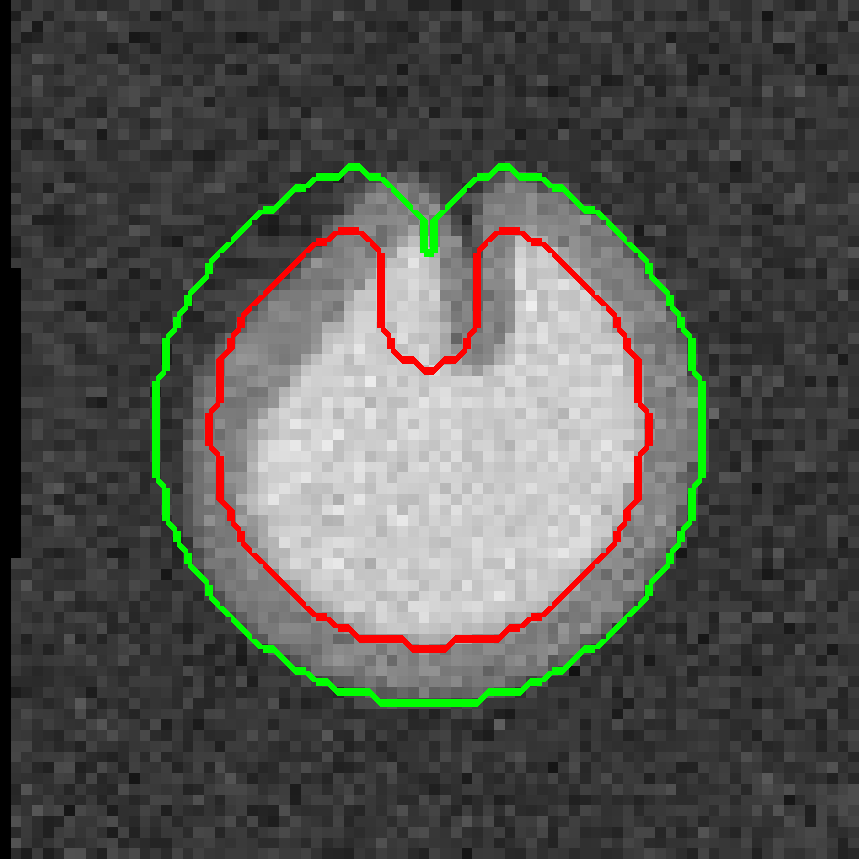
\includegraphics[width=0.19\textwidth]{model2result_b_1} &
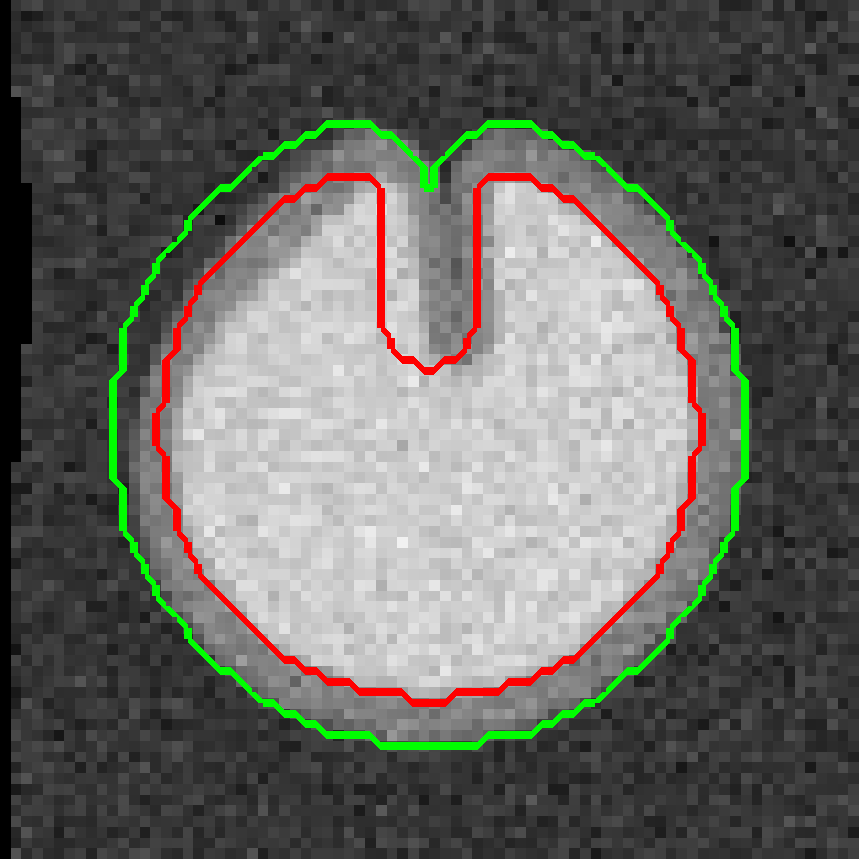
\includegraphics[width=0.19\textwidth]{model2result_b_2} &
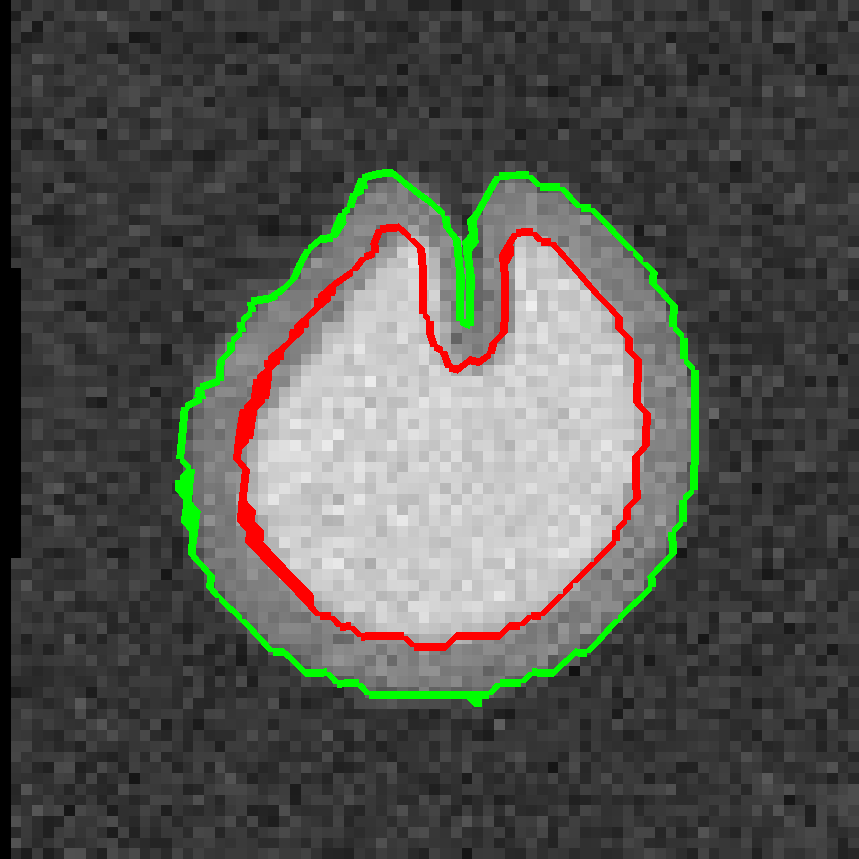
\includegraphics[width=0.19\textwidth]{model2result_a_1} &
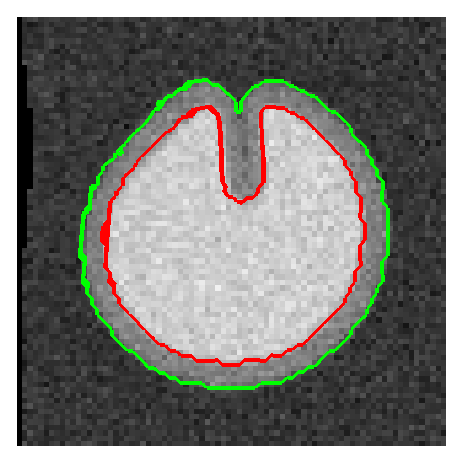
\includegraphics[width=0.19\textwidth]{model2result_a_2} &
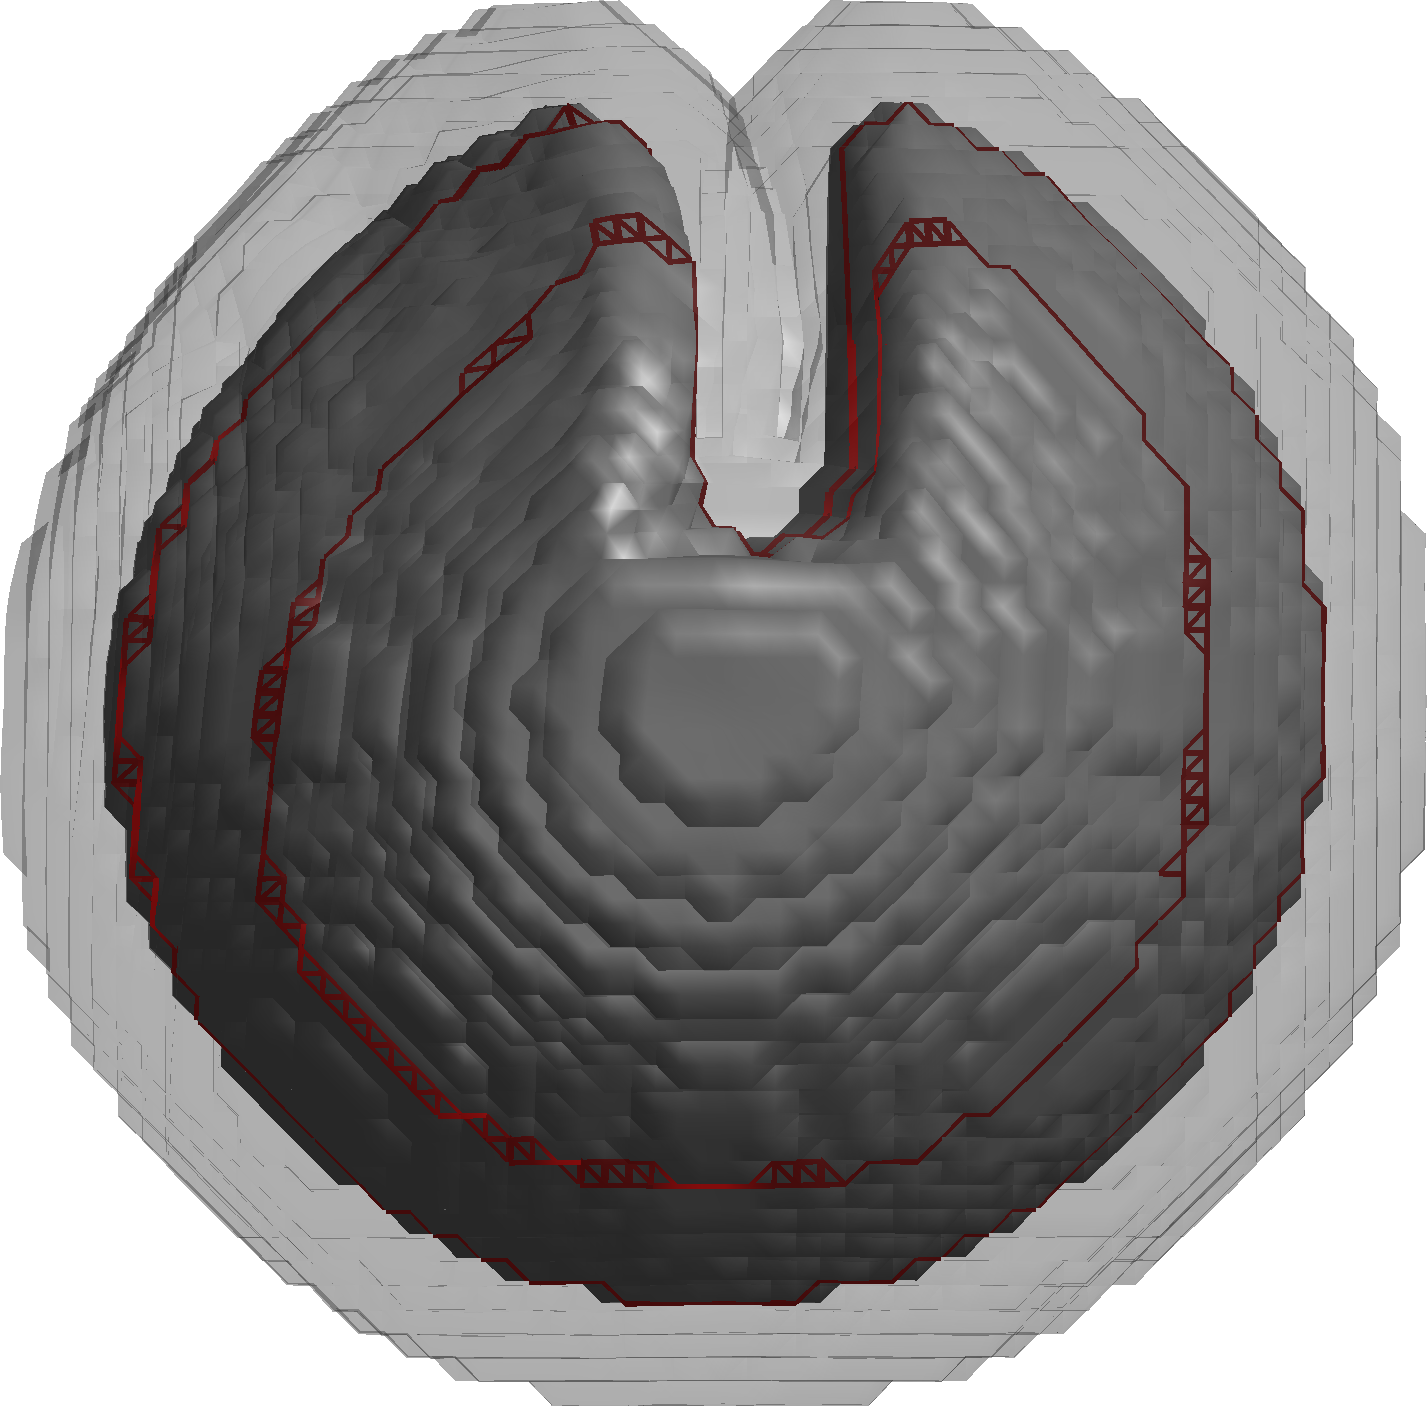
\includegraphics[width=0.19\textwidth]{model2surf} \\
\multicolumn{2}{c}{a)} & \multicolumn{2}{c}{b)} & c)
\end{tabular}
\caption{Result of the segmentation performance on the sulcus model.
a) Two slices and prior contours before segmentation-registration. b) The same slices and contours after distortion estimation. c) 3D rendering of the deformed priors, with the traces of the two selected slices highlighted. 
%In red and blue colors the obtained \gls{wm}/\gls{gm} 
%and \gls{gm}/\gls{csf} contours for the deformed image, respectively.
%In white color, the initial shape priors for the \gls{wm}/\gls{gm}
%interface.
{\color{red}{This figure is to be replaced by the real result,
this is a proof of concept of registration that does not solve
the pv problem. The current figure also removes the outer prior}}}
\label{fig:sulcusmodel_result}
\end{figure}


\subsection{Simulated diffusion data}
%
The proposed method successfully reverted the synthetic distortion
field we applied to the data. With 16x16x16 control points, the
displacements field is dense enough to correctly represent the
synthetic field. Second row in \autoref{fig:fa} shows the fitted
contours obtained by using the original surfaces of the model
as shape priors, with a constant translation of (5.0mm,10mm.,-5.0mm)
to illustrate briefly the extent of the capture range of the algorithm.
Computation time in this case was around 4 minutes in the previously
described platform. \\
%

\begin{figure}
\begin{tabular}{ccccc}
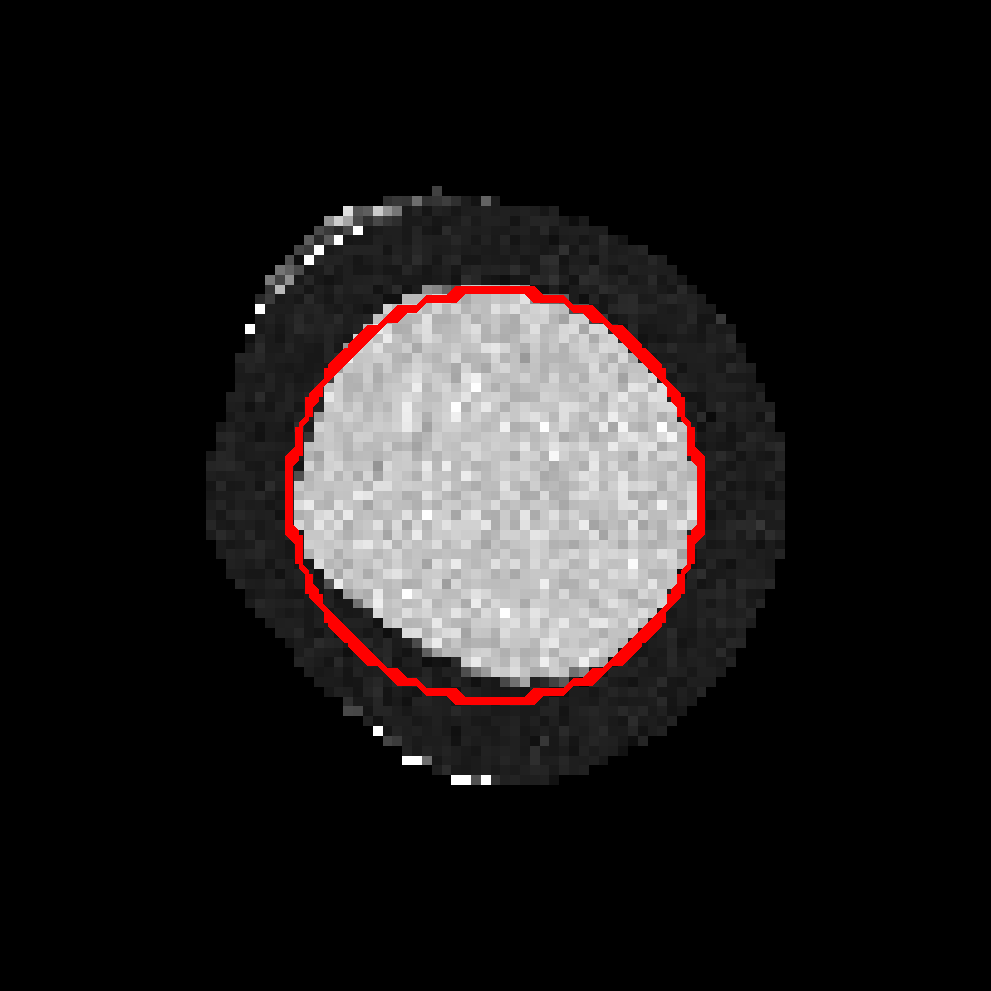
\includegraphics[width=0.19\textwidth]{model1result_b_1} &
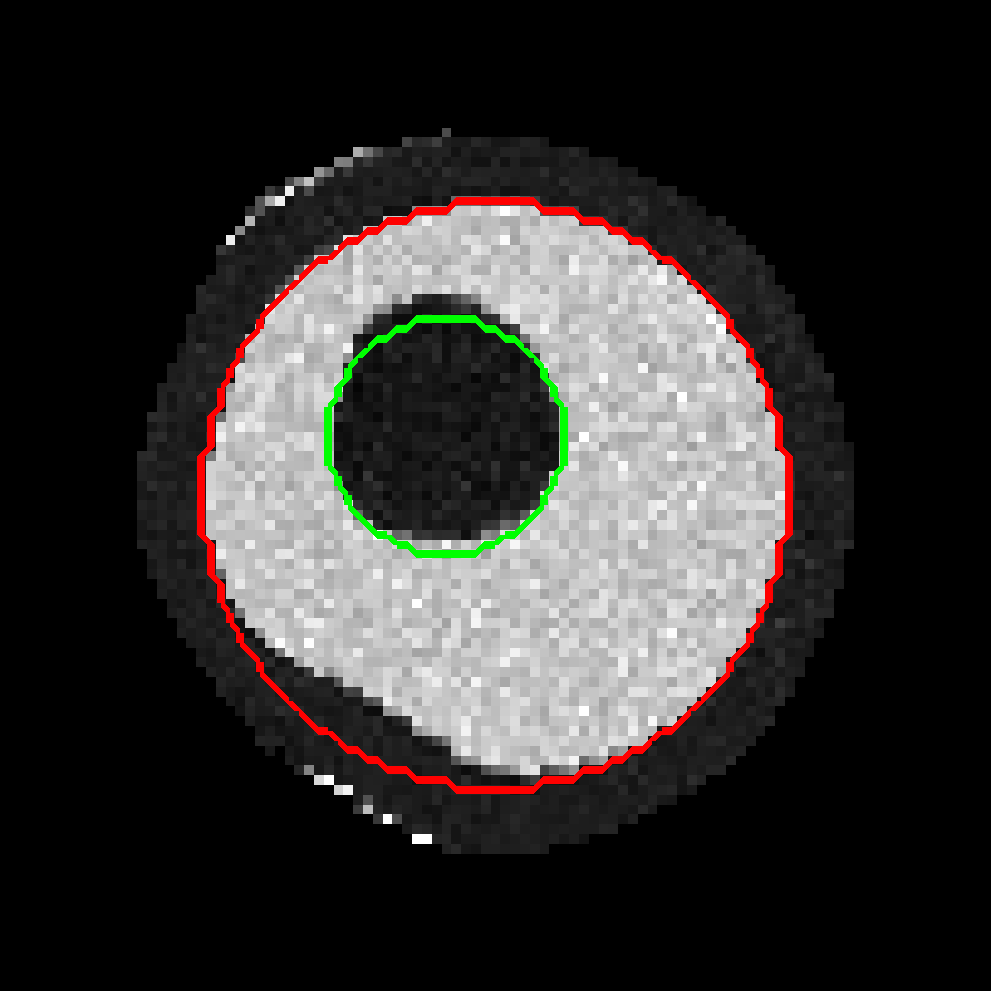
\includegraphics[width=0.19\textwidth]{model1result_b_2} &
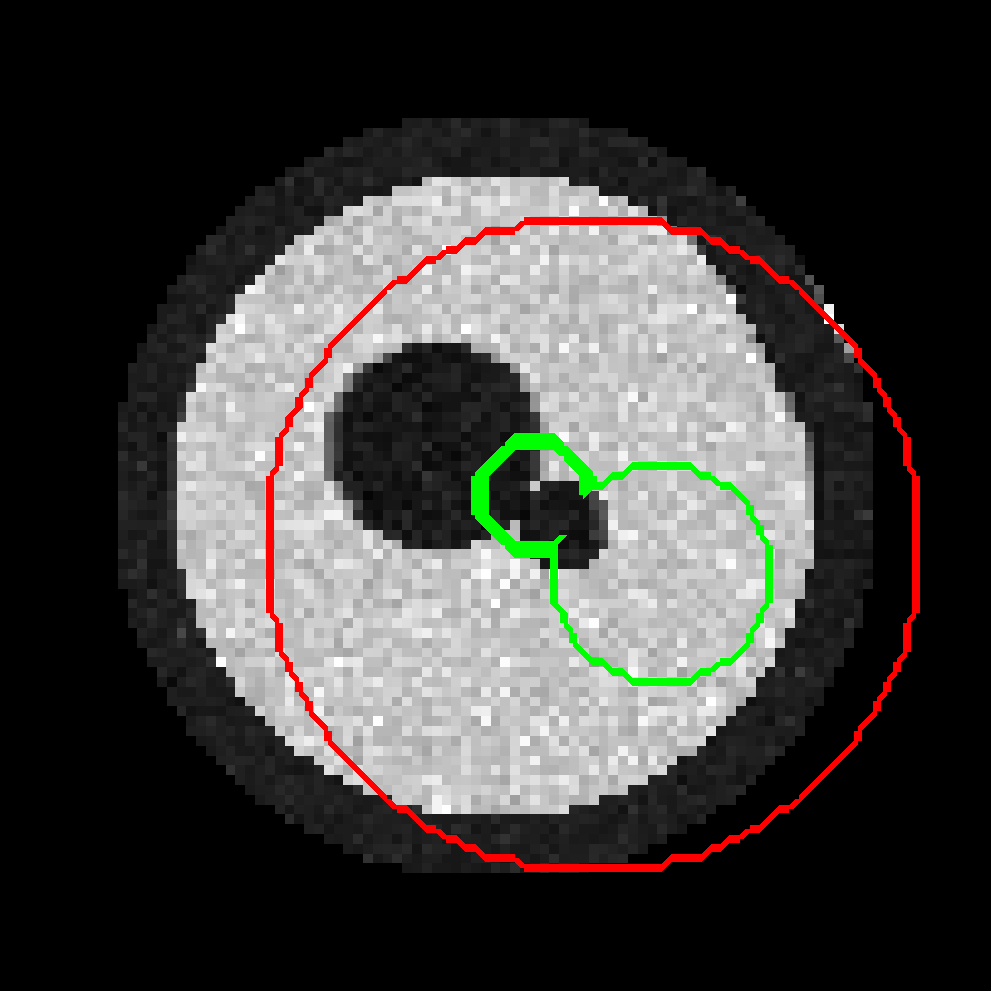
\includegraphics[width=0.19\textwidth]{model1result_b_3} &
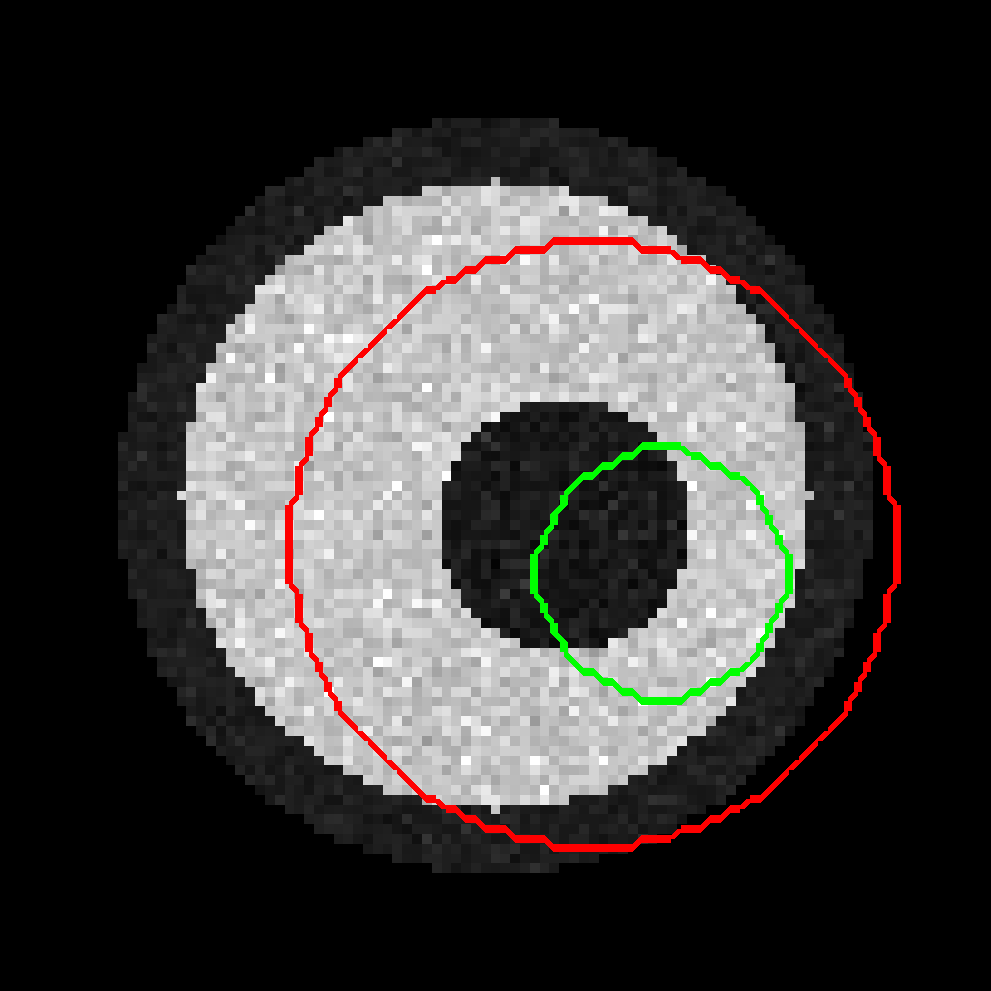
\includegraphics[width=0.19\textwidth]{model1result_b_4} &
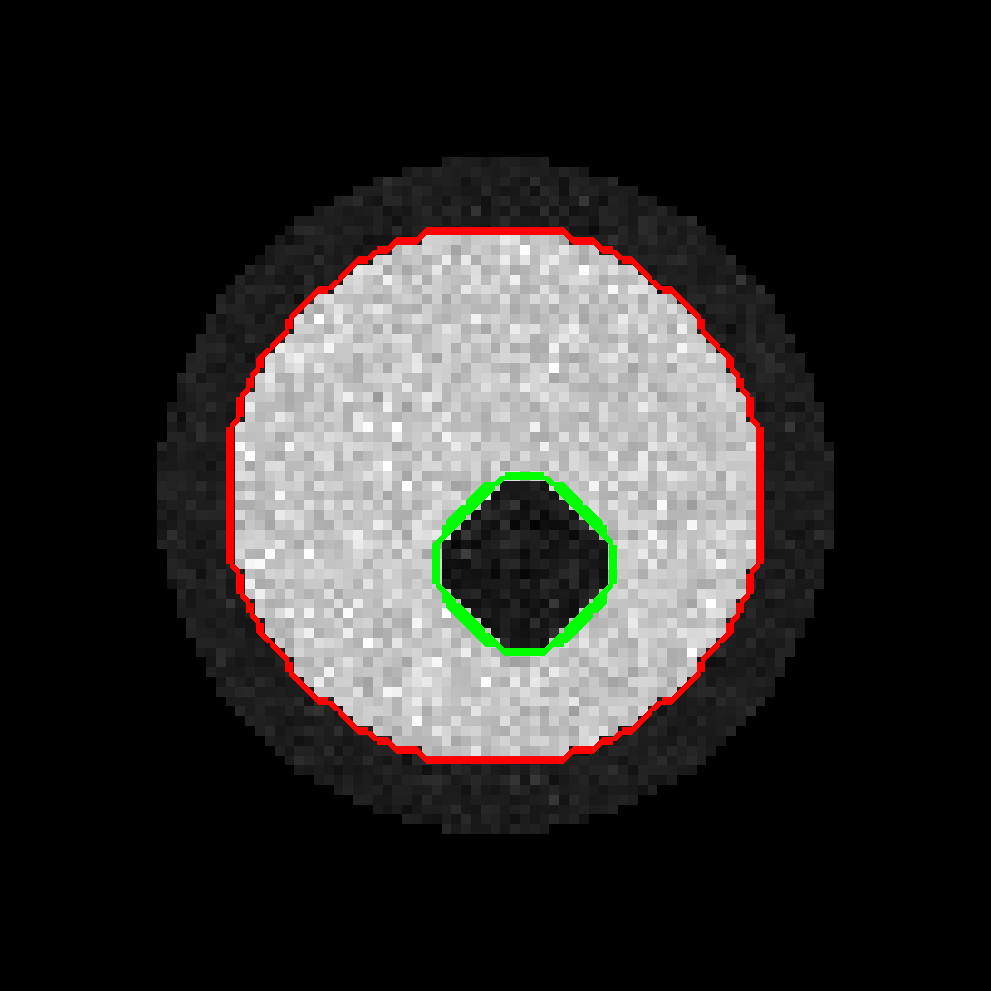
\includegraphics[width=0.19\textwidth]{model1result_b_5} \\
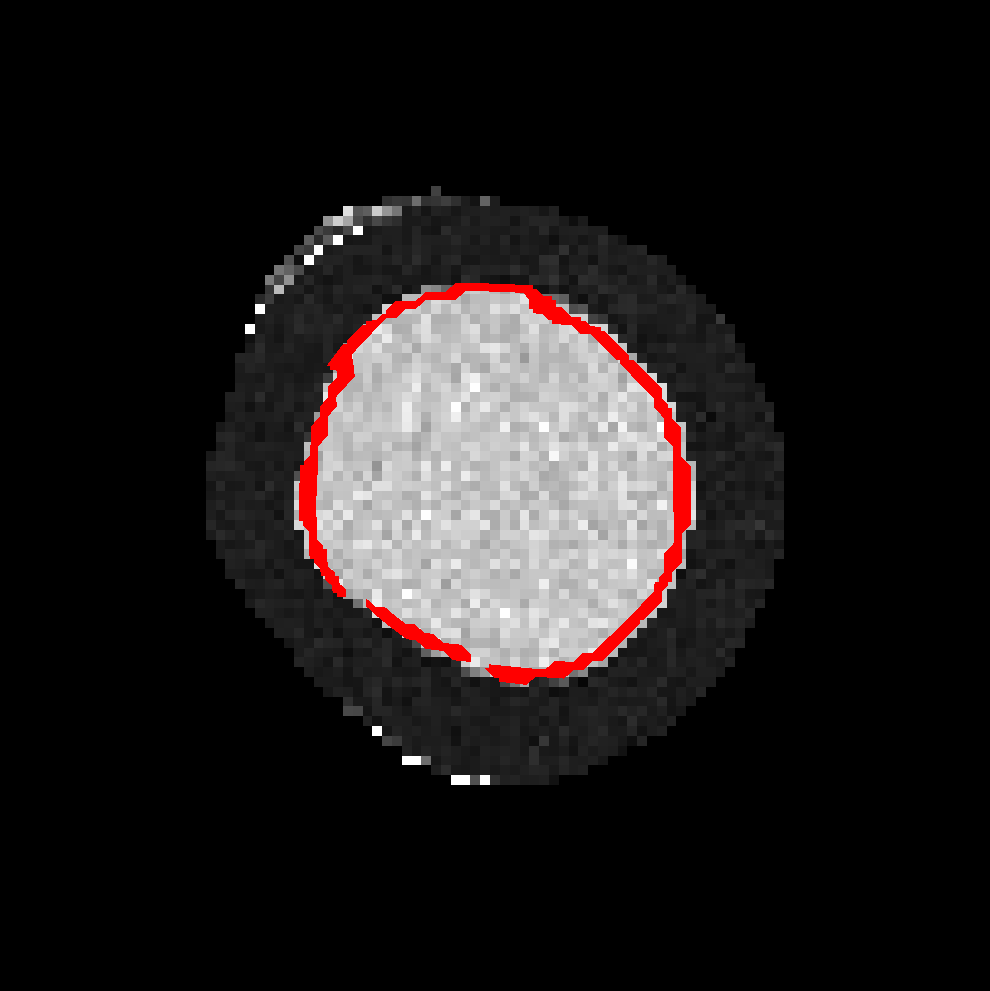
\includegraphics[width=0.19\textwidth]{model1result_a_1} &
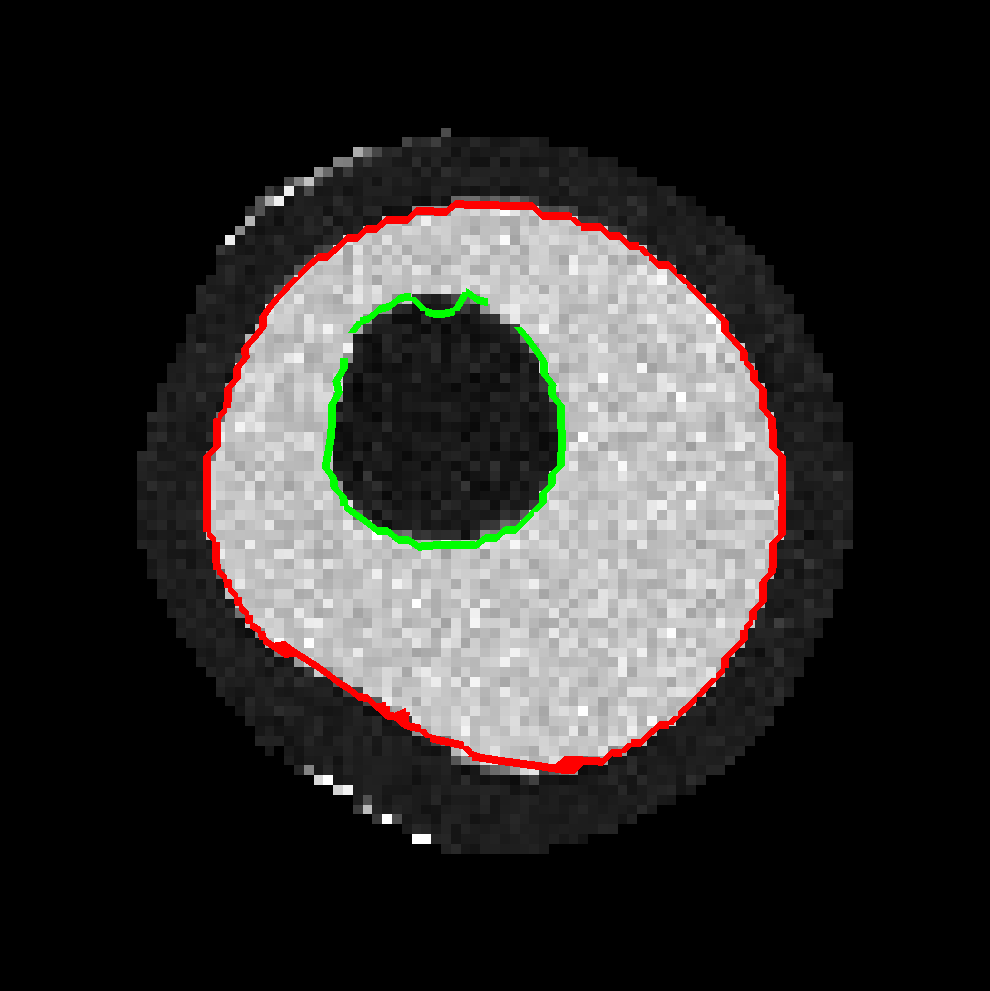
\includegraphics[width=0.19\textwidth]{model1result_a_2} &
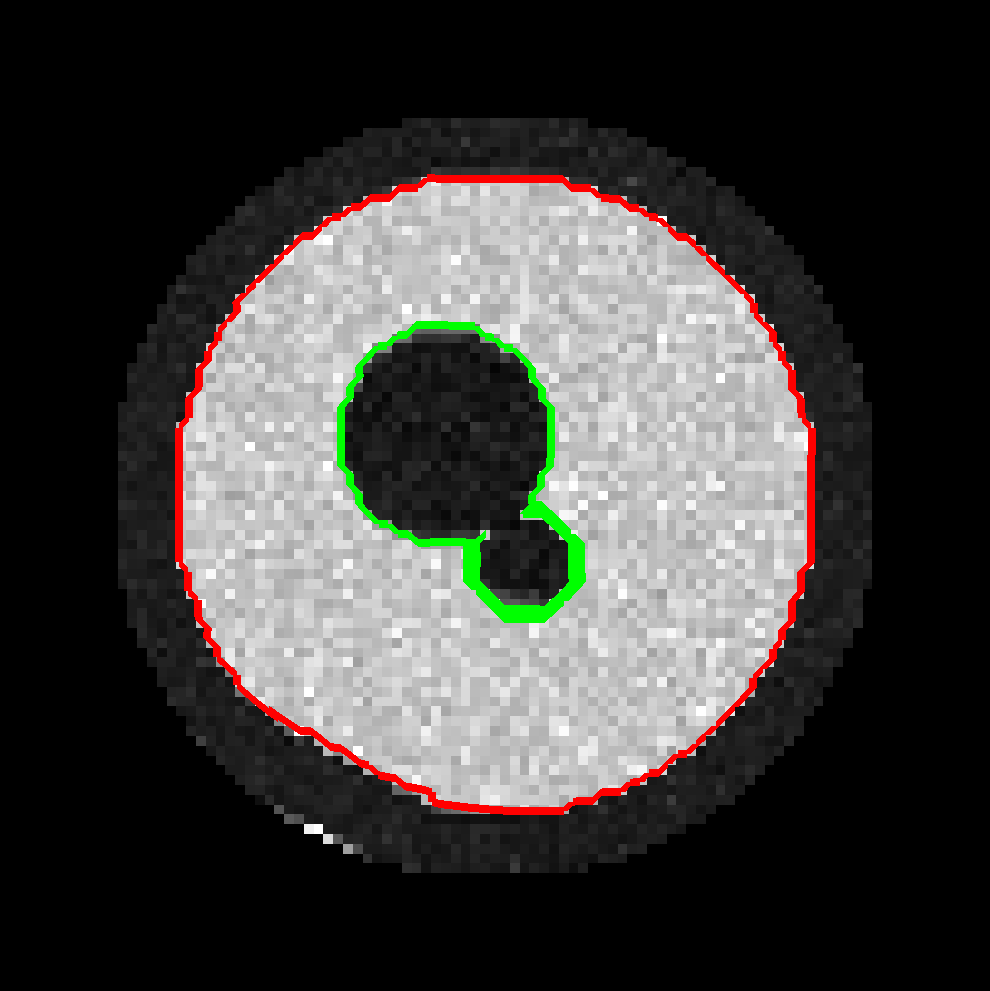
\includegraphics[width=0.19\textwidth]{model1result_a_3} &
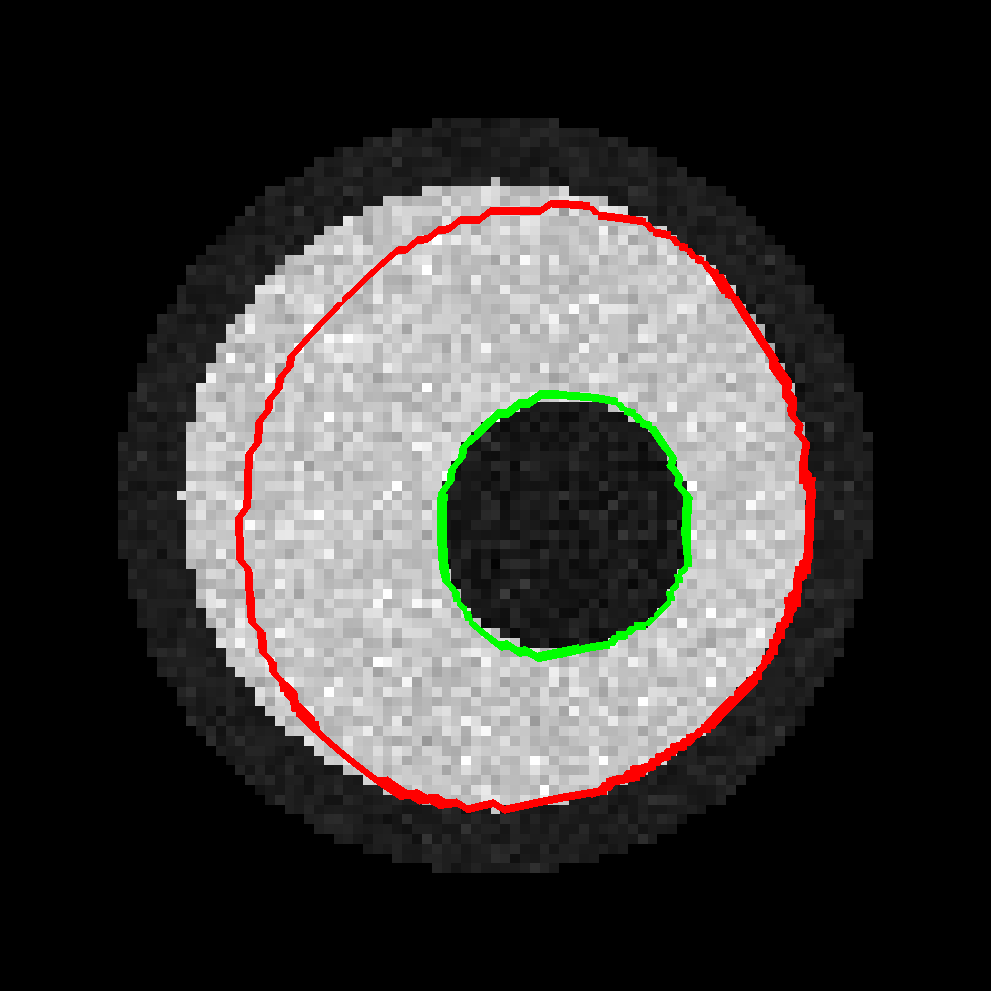
\includegraphics[width=0.19\textwidth]{model1result_a_4} &
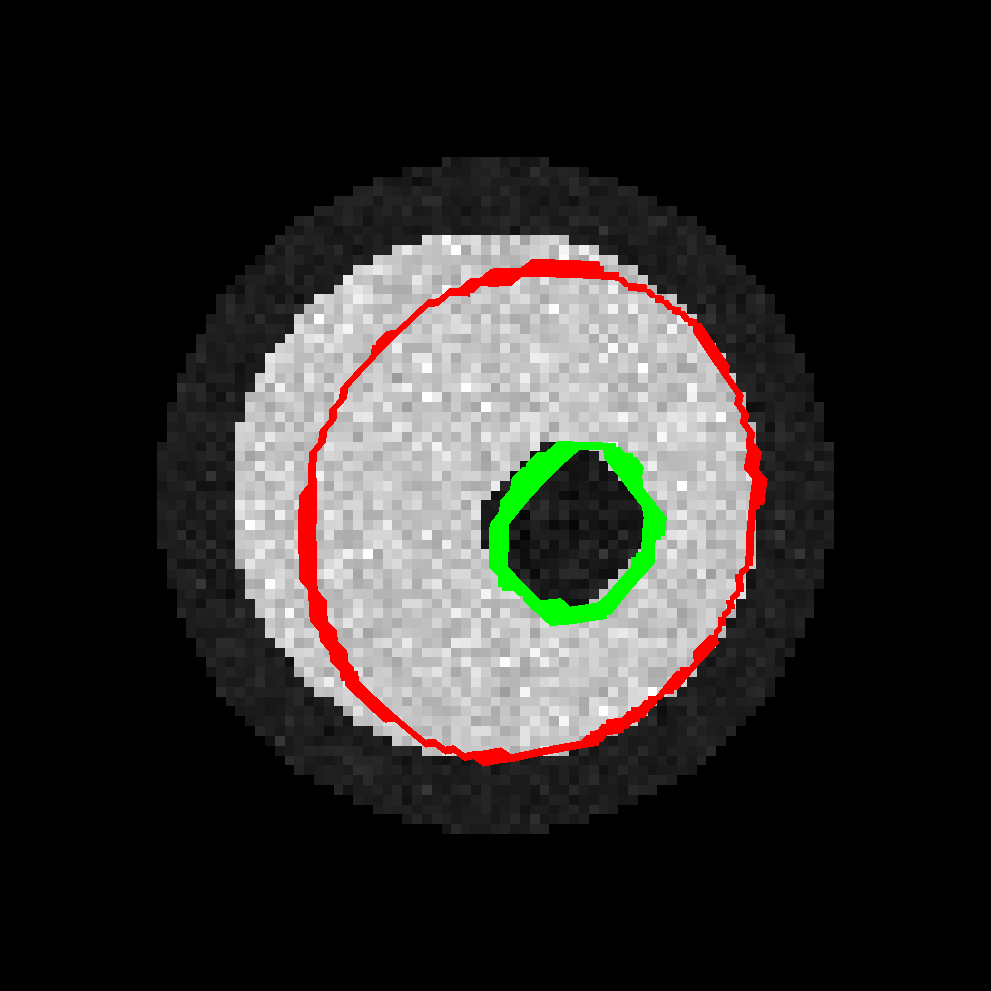
\includegraphics[width=0.19\textwidth]{model1result_a_5} \\
\end{tabular}
\caption{First row presents several slices along Z axis of the distorted \gls{fa} map and
the undistorted \gls{wm}-\gls{gm} and \gls{wm}-\gls{csf} contours given as shape priors. Second row contains the same map, now with the contours after joint segmentation-registration.}
\label{fig:fa}
\end{figure}